\vspace{-4ex}
\section{Introduction}
\vspace{-1ex}

Recent studies have demonstrated that large language models (LLMs) are capable of tackling mathematical problems~\citep{qwq-32b-preview,qwen2.5,o1,deepseekv3}. However, the conventional approach of having LLMs generate complete solutions in a single inference -- akin to System 1 thinking~\citep{thinking} -- often yields fast but error-prone results~\citep{valmeekam2023planning,gpt4}. In response, test-time compute scaling~\citep{snell2024scaling,rstar} suggests a paradigm shift toward a System 2-style thinking, which emulates human reasoning through a slower and deeper thought process. In this paradigm, an LLM serves as a policy model to generate multiple math reasoning steps, which are then evaluated by another LLM acting as a reward model~\citep{o1}. The steps and solutions deemed more likely to be correct are selected. The process repeats iteratively and ultimately derives the final answer.



In the test-time compute paradigm, the key is to train a powerful policy model that generates promising solution steps and a reliable reward model that accurately evaluates them, both of which depend on \emph{high-quality} training data. Unfortunately, it is well-known that off-the-shelf high-quality math reasoning data is scarce, and synthesizing high-quality math data faces fundamental challenges. 
For the policy model, it is challenging to distinguish erroneous reasoning steps from the correct ones, complicating the elimination of low-quality data. It is worth noting that in math reasoning, a correct final answer does not ensure the correctness of the entire reasoning trace~\citep{lanham2023measuring}. Incorrect intermediate steps significantly decrease data quality.  
As for the reward model, process reward modeling (PRM) shows a great potential by providing fine-grained feedback on intermediate steps~\citep{lightman2023let}. However, the training data is even scarcer in this regard: accurate step-by-step feedback requires intense human labeling efforts and is impractical to scale, while those automatic annotation attempts show limited gains due to noisy reward scores~\citep{luo2024improve,mathshepherd,alphamath}. 
Due to the above challenges, existing distill-based data synthesis approaches to training policy models, e.g., scaling up GPT4-distilled CoT data~\citep{mathscale,o1journeypart2}, have shown diminishing returns and cannot exceed the capability of their teacher model; meanwhile, as of today, training reliable PRMs for math reasoning remains an open question.




\begin{figure*}[t]
	\centering
	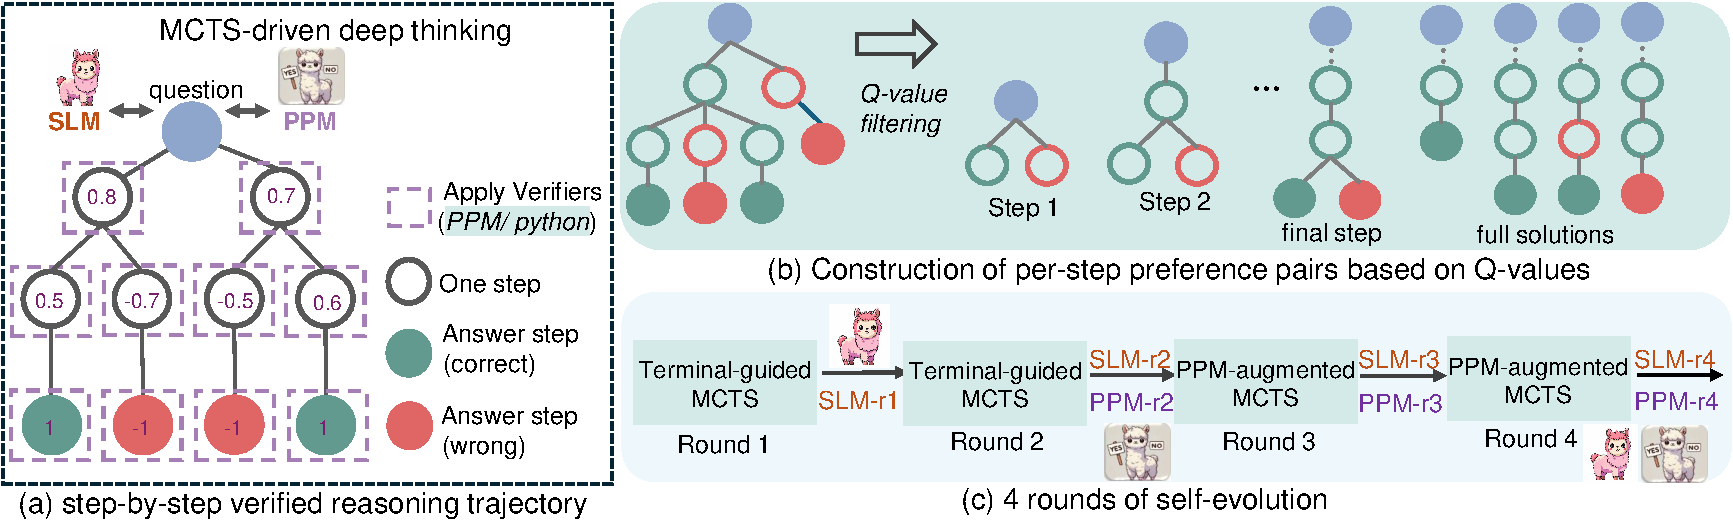
\includegraphics[width=1\textwidth]{method_final.pdf}	
	\vspace{-4ex}
	\caption{The overview of {\sysname}.}
	\label{fig:method}
\end{figure*}

In this work, we introduce \textbf{\sysname}, a self-evolvable System 2-style reasoning approach that achieves the state-of-the-art math reasoning, rivaling and sometimes even surpassing OpenAI o1 on challenging math competition benchmarks with a model size as small as 7 billion. Unlike solutions relying on superior LLMs for data synthesis, {\sysname} leverages smaller language models (SLMs) with Monte Carlo Tree Search (MCTS) to establish a self-evolutionary process, iteratively generating higher-quality training data. To achieve self-evolution, {\sysname} introduces three key innovations. 

First, a novel code-augmented CoT data synthesis method, which performs \textit{extensive} MCTS rollouts to generate \textit{step-by-step verified reasoning trajectories} with \textit{self-annotated MCTS Q-values}. Specifically, math problem-solving is decomposed into multi-step generation within MCTS. At each step, the SLM serving as the policy model samples candidate nodes, each generating a one-step CoT and the corresponding Python code. To verify the generation quality, only nodes with successful Python code execution are retained, thus mitigating errors in intermediate steps. Moreover, extensive MCTS rollouts automatically assign a Q-value to each intermediate step based on its contribution: steps contributing to more trajectories that lead to the correct answer are given higher Q-values and considered higher quality. This ensures that the reasoning trajectories generated by SLMs consist of correct, high-quality intermediate steps.



Second, a novel method that trains an SLM acting as a \textit{process preference model}, i.e., a PPM to implement the desired PRM, that reliably predicts a reward label for each math reasoning step. The PPM leverages the fact that, although Q-values are still not precise enough to score each reasoning step despite using extensive MCTS rollouts, the Q-values can reliably distinguish positive (correct) steps from negative (irrelevant/incorrect) ones. Thus the training method constructs preference pairs for each step based on Q-values and uses a pairwise ranking loss~\citep{instructgpt} to optimize PPM's score prediction for each reasoning step, achieving reliable labeling. This approach avoids conventional methods that directly use Q-values as reward labels~\citep{luo2024improve,alphamath}, which are inherently noisy and imprecise in stepwise reward assignment.




Finally, a four-round self-evolution recipe that progressively builds both a frontier policy model and PPM from scratch. We begin by curating a dataset of 747k math word problems %with ground-truth labels 
from publicly available sources. In each round, we use the latest policy model and PPM to perform MCTS, generating increasingly high-quality training data using the above two methods to train a stronger policy model and PPM for next round. Each round achieves progressive refinement: (1) a stronger policy SLM, (2) a more reliable PPM, (3) generating better reasoning trajectories via PPM-augmented MCTS, and (4) improving training data coverage to tackle more challenging and even competition-level math problems.




Extensive experiments across four SLMs (1.5B-7B) and seven math reasoning tasks demonstrate the effectiveness of {\sysname}. Remarkably, {\sysname} improves all four SLMs, matching or even surpassing OpenAI o1 on challenging math benchmarks. On MATH benchmark, with 8 search trajectories, {\sysname} boosts Qwen2.5-Math-7B from 58.8\% to 89.4\% and Qwen2.5-Math-1.5B from 51.2\% to 87.8\%. With 64 trajectories, the scores rise to 90\% and 88.4\%, outperforming o1-preview by 4.5\% and 2.6\% and matching o1-mini's 90\%. On the Olympiad-level AIME 2024, {\sysname} solves on average 53.3\% (8/15) of the problems, exceeding o1-preview by 8.7\% and all other open-sourced LLMs. We further conduct comprehensive experiments to verify the superiority of step-by-step verified reasoning trajectories over state-of-the-art data synthesis baselines, as well as the PPM's effectiveness compared to outcome reward models and Q value-based PRMs. Finally, we present key findings from {\sysname} deep thinking, including the intrinsic self-reflection capability and PPM's preference for theorem-applications intermediate steps.  























